
\section{The A* Algorithm}

The A* algorithm is a solution to the single source shortest path problem. It is applied on a graph (directed or undirected) with various costs for all the edges of the graph. A* finds the path of edges from a given source and goal node that minimizes the total sum of the edge costs.
\newline\newline
It improves on algorithms like Dijkstra's algorithm by using a heuristic to help guide the search for the end goal. Every node $n$ in the set of vertices $V$ has a distance $g(n)$ from the source node that was discovered by exploring the different paths from the start to $n$. There is also a heuristic function $h$ such that $h(n)$ represents an estimate of the remaining distance to the goal node. Nodes on the frontier of the search are placed on a priority queue. They are then picked to be explored from the frontier based on a combination of the cost and heuristic functions: 
$$f(n) = g(n) + h(n)$$
By using $f(n)$ to prioritize nodes that we believe are more likely to reach the goal faster, we are able to expand fewer nodes and find the least cost path more efficiently then Dijkstra's algorithm.
\newline\newline
In order to ensure that we have an accurate estimate of the priority of a node, we need our heuristic to be consistent in order for the A* algorithm to generate a provably correct output. A heuristic is consistent if for a node $s$ and any of its neighbors $s'$, it satisfies the following inequality:
$$f(s) \le d(s, s') + f(s')$$
where $d(s, s')$ is the distance between the two nodes.

\begin{figure}
    \centering
    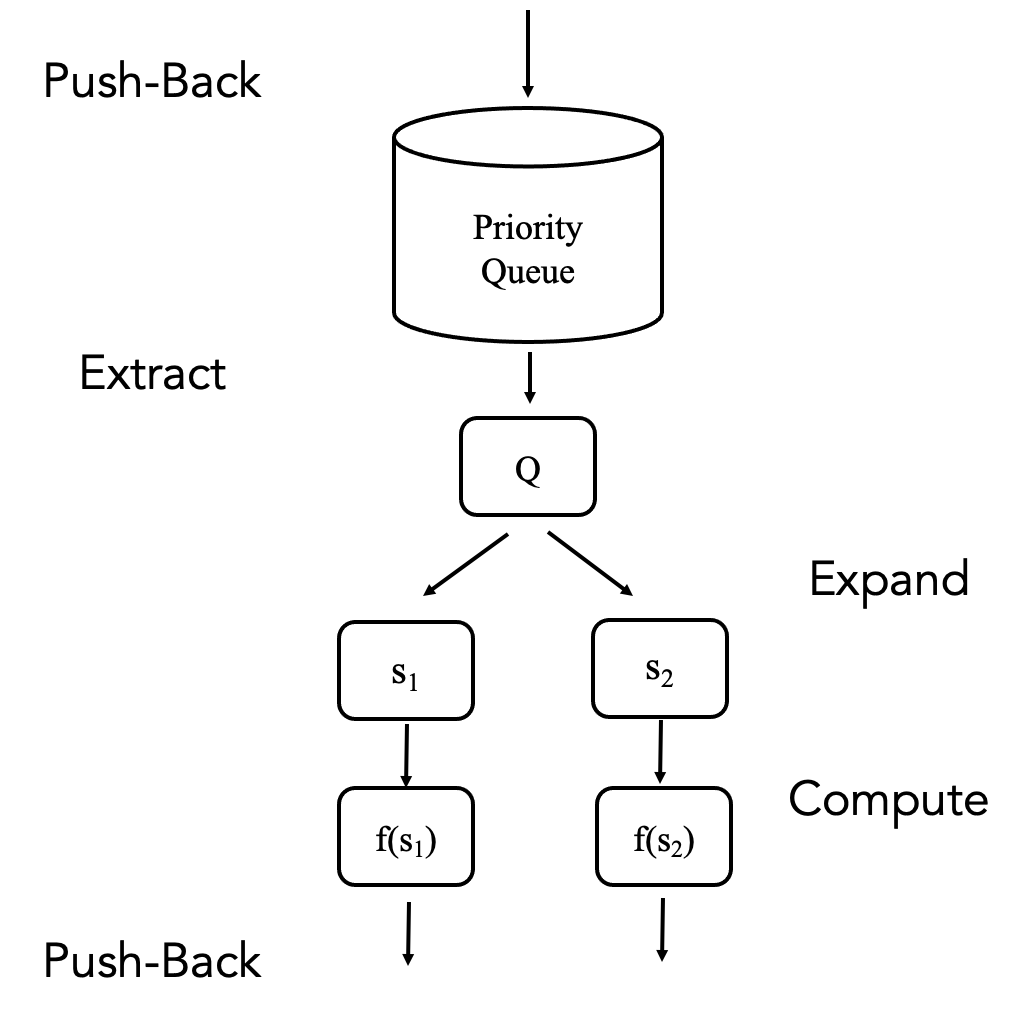
\includegraphics[scale=0.5]{figures/astar.png}
    \caption{A* workflow}
    \label{fig:astar}
\end{figure}

\section{Algorithm (GA*)\cite{paper}}

The A* algorithm as described above is \textbf{not amenable to parallelization}. The priority queue requires that only the topmost entry in the priority queue be used for exploration. As a result, it is not possible to create a parallel version of the algorithm described above without changing the data structures.\newline\newline
GA* is a general version of A* that can be run in a parallel setting. We present the pseudocode of our algorithm below:

\begin{verbatim}
let GA start target =
    let Q = {q1, q2, ..., qk}       // set of priority queues (open list)
    let H = {}                      // global hash table (close list)
    let m = None                    // state pointer (found goal)
    
    q1.push(start)
    while not all q in Q empty do
        let S = []                  // global list (expanded states)
        
        parallel for i in [0, k] do
            if qi empty then break
            
            // every thread expands one state
            let si = qi.pop()
            
            // update goal state if found state is shorter path to goal
            if si = t then
                if m = None or si.total_cost < m.total_cost then
                    m <- si
                break
            
            // add neighbors
            S.extend(s' for s' in s.next)
        done
        
        // check if found goal state is closer than all other states
        if m != None and m.total_cost <= min si.total_cost then return m.path
        
        // remove expanded states that have already been seen cheaper
        parallel for i in [0, s.length] do
            if si in H and H[si] < si.path_cost then s.pop(i)
        done
        
        parallel for i in [0, s.length] do
            // push si to some q in Q evenly
            Q.push(si)
            
            // store seen expanded paths
            H[si] <- si.path_cost
        done
    done
    return m

\end{verbatim}
At a high level, this algorithm uses \textbf{multiple priority queues} to generate a path between the start state and goal state. An explicit graph data structure is unnecessary in this scenario as we can determine neighbor states from the current state (and anyways, an explicit graph structure would be very much too large in scenarios that would motivate parallelization on this scale).\newline\newline
The pseudocode is commented at each step, but the high level idea is that each thread has its own priority queue of states. Each thread expands the top node of its own priority queue, checks if it has reached a goal state and if it has been visited already and expands the neighbors of this state.\newline\newline
When states are expanded, the number of states grows exponentially, resulting in a smoothing of the states distribution across all of the threads. This results in \textbf{state duplication} among independent threads that may separately want to push the same state onto the frontier. To handle this, we need to keep track of which nodes have been explored and/or will be on the frontier. We utilize the global hash table (described below) for this purpose.

\section{Data Structures}

\begin{figure}
    \centering
    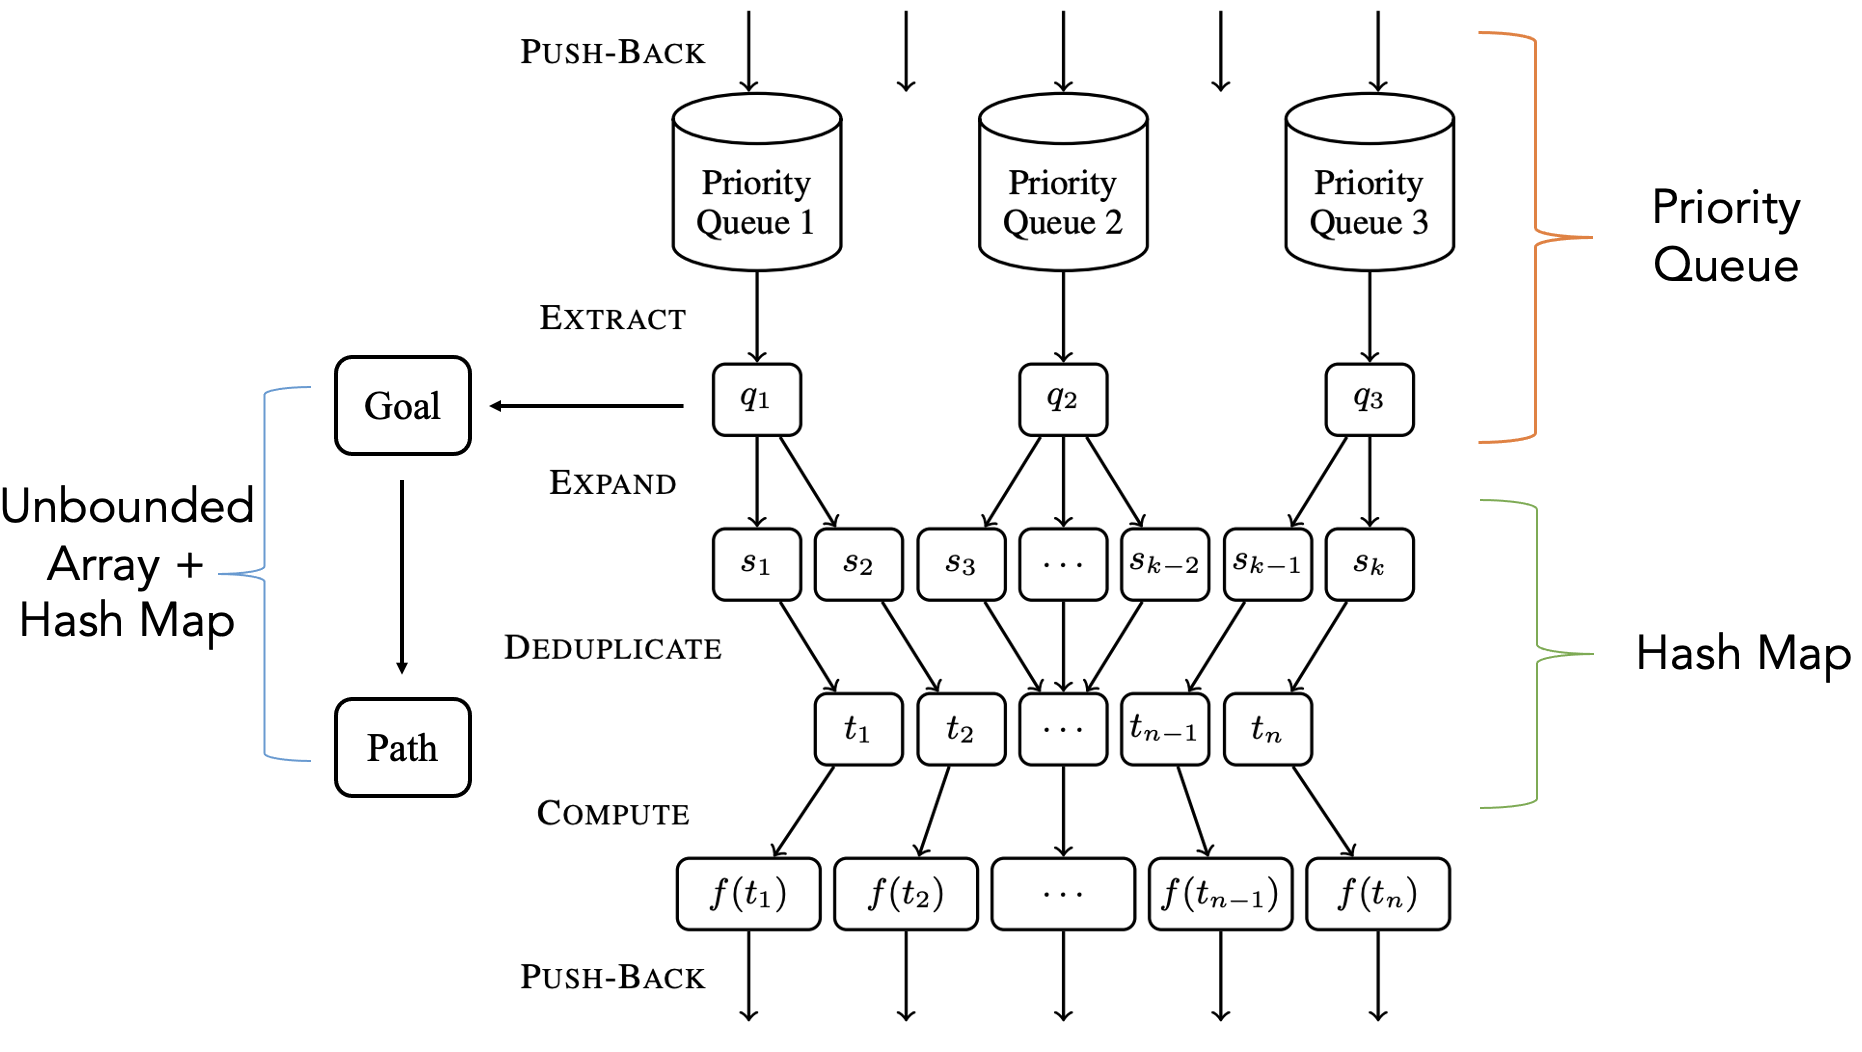
\includegraphics[scale=0.5]{figures/gastar_ds.png}
    \caption{GA* workflow with relevant data structures (based on \cite{paper})}
    \label{fig:gastar_ds}
\end{figure}

\subsection{Serial}
Standard libraries cannot be used in CUDA code due to GPU memory working differently than CPU memory. Thus, certain serial data structures need to be re-implemented to accommodate for this.
\subsubsection{Unbounded Array}
This structure is used to generate the path to the goal state once the algorithm terminates. Thus, unlike a standard unbounded array, it only requires a \texttt{push} operation. It has a growth factor of $2$ (resize to double its original size).
\subsubsection{Priority Queue (Heap)}
Every thread contains their own priority queue for expanding states. These are min-heaps (for retrieving closest perceived state) that operate on top of an unbounded array structure (same as above, but with a shrinkage factor of $2$ as well). In accordance with the above algorithm, they have \texttt{pop}, \texttt{push}, and \texttt{is\_empty} operations.
\subsection{Parallel}
\subsubsection{Hash Table (Parallel Hashing with Replacement)\cite{paper}}
This structure is used to keep a global collection of visited states and their path costs. Because of this global attribute, this is the bottleneck in the algorithm. A standard hash table contains an unbounded array of linked lists, but the structure's dynamic nature (on item inserts) makes it extremely difficult to parallelize. To tackle this problem, we implement parallel hashing with replacement\cite{paper} which uses a static list and multiple hash functions. The second hash function can search for new locations in the table for a node if another element collides with it in the first hash function. Our rationale for choosing this structure is explored in the Approach chapter. As in a standard hash table, this has assignment, existence, and modification operations. These operations are allowed to run in parallel with one another and must be thread-safe.

\section{Workload}
In the sequential algorithm for A*, a single priority queue is used to determine the next state to extract. Since node neighbors are fully dependent on the nodes within the priority queue, this data structure becomes the bottleneck if we were to parallelize the algorithm. If instead (as demonstrated in the pseudocode), we allow for states to be expanded independently of one another using multiple independent priority queues, we will allow for duplicate expansions. Thus, especially for large problem spaces, the approach is massively parallel.\newline\newline
Since each thread operates independently in the sense that they expand nodes without dependencies on nodes held by other threads, \textbf{this program is task parallel}. Locality and vector instructions are not as relevant due to this.